\pagestyle{azougue}
\label{azougue}


\begin{textblock*}{5.625in}(0pt,0pt)%
\vspace*{-1.45cm}
\hspace*{-1.2cm}\includegraphics*[width=112mm]{./imgs/AZOUGUE.png}
\end{textblock*}

\pagebreak

\hspace{.5cm}

\begin{center}
\hspace*{-.5cm}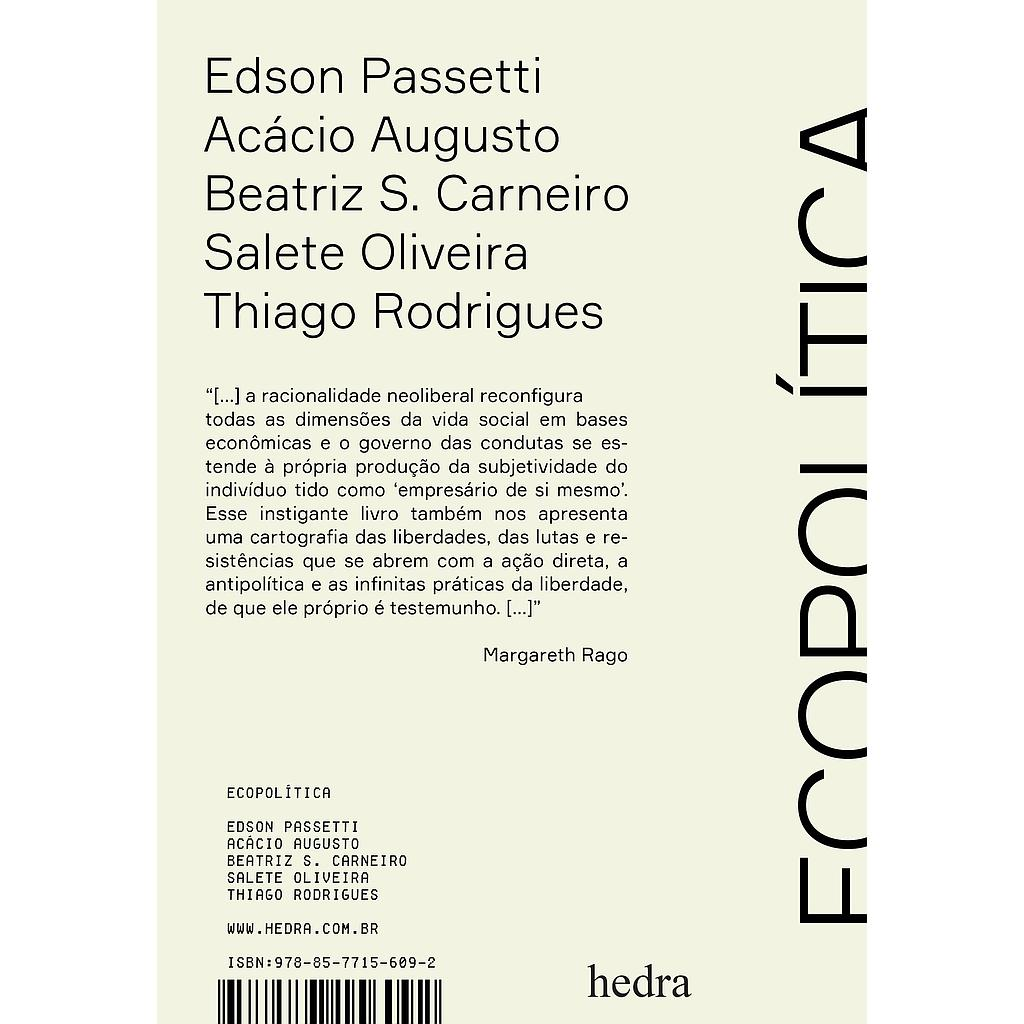
\includegraphics[width=70mm]{eco.jpeg}
\end{center}

\hspace*{-2cm}\_\_\_\_\_\_\_\_\_\_\_\_\_\_\_\_\_\_\_\_\_\_\_\_\_\_\_\_\_\_\_\_\_\_\_\_\_\_\_\_\_\_\_\_\_\_\_\_\_\_\_\_\_\_\_\_\_\_\_\_\_\_\_\_\_\_\_\_\_\_\_\_\_\_

\medskip

\noindent{}Lorem ipsum dolor sit amet, consectetur adipiscing elit.
Donec sodales tortor a purus accumsan, ut ultricies purus
maximus. Aliquam bibendum consequat mi, sed commo-
do velit pellentesque id. Vivamus ultricies ligula in semper
sagittis. Donec mollis odio in lectus tristique, sed convallis
est interdum. Cras eget sem condimentum, pretium purus
eu, auctor.

\hspace{.5cm}

\hspace*{-.4cm}\begin{minipage}[c]{0.90\linewidth}
\small{
{\Formular{\textbf{
\hspace*{-.1cm}Título: Weber (Frankfurt 2)\\
Autor: Gabriel Cohn\\ 
Editora: Azougue\\
Páginas: 320\\
Formato: 17x24cm\\
Preço: R\$ 89,90\\
ISBN: ?????????
}}}}
\end{minipage}

\pagebreak

\hspace{.5cm}

\begin{center}
\hspace*{-1cm}\raisebox{5.5cm}{\rotatebox[origin=t]{90}{\Formular{\textbf{Lançamento}}}}
\hspace*{1cm}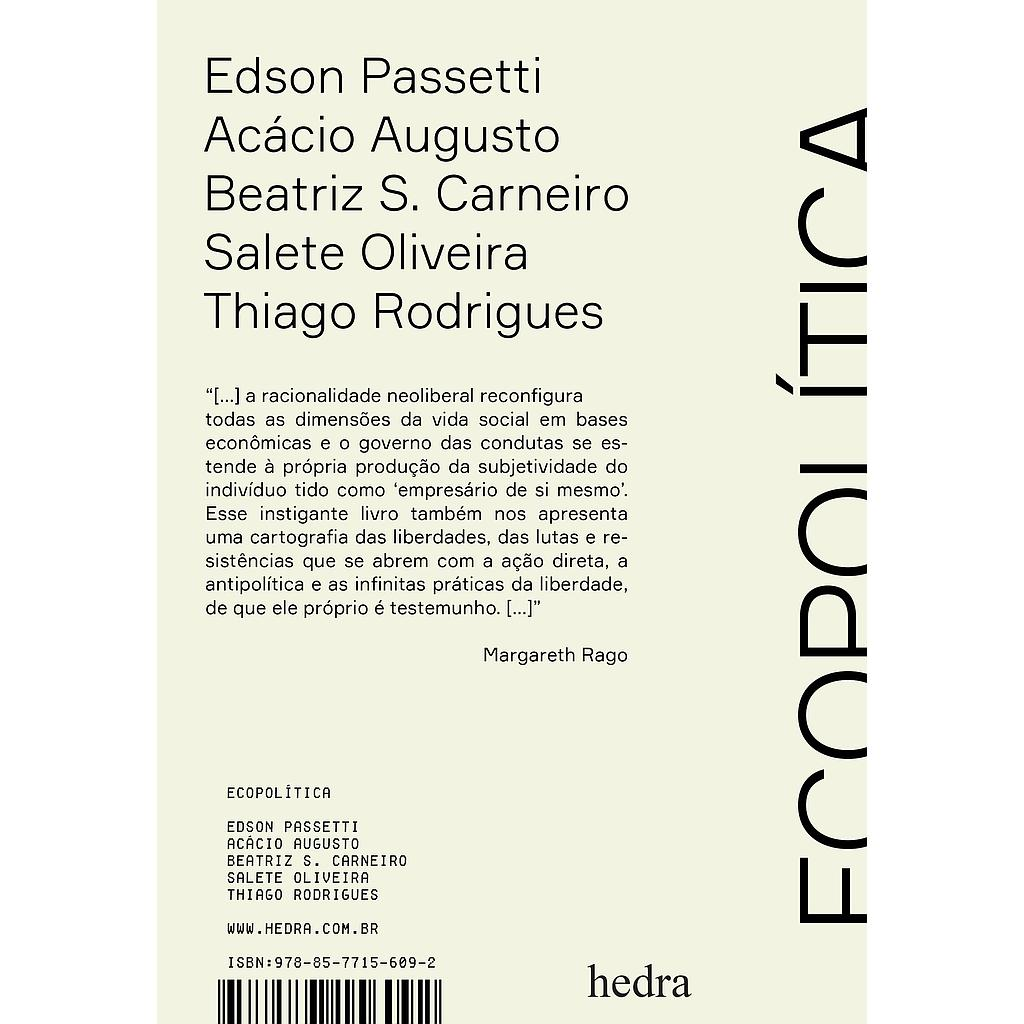
\includegraphics[width=70mm]{eco.jpeg}
\end{center}

\hspace*{-2cm}\_\_\_\_\_\_\_\_\_\_\_\_\_\_\_\_\_\_\_\_\_\_\_\_\_\_\_\_\_\_\_\_\_\_\_\_\_\_\_\_\_\_\_\_\_\_\_\_\_\_\_\_\_\_\_\_\_\_\_\_\_\_\_\_\_\_\_\_\_\_\_\_\_\_

\medskip

\noindent{}{\slsc{Hotel Universo}} traz uma antologia e uma análise do cancioneiro e da lírica de Ronaldo Bastos, realizada por Marcos Lacerda, importante crítico musical da nova geração. Um dos principais compositores da canção brasileira, Ronaldo Bastos foi um dos criadores do Clube da Esquina, que teve como expoentes artistas do porte de Milton Nascimento e Lô Borges, e suas canções foram gravadas por nomes como Caetano Veloso, Elis Regina e Tom Jobim.

\hspace{.5cm}

\hspace*{-.4cm}\begin{minipage}[c]{0.90\linewidth}
\small{
{\Formular{\textbf{
\hspace*{-.1cm}Título: Hotel Universo – a poética de Ronaldo Bastos\\
Autor: Marcos Lacerda\\ 
Editora: Azougue\\
Páginas: 174\\
Formato: 14x21cm\\
Preço: R\$ 39,00\\
ISBN: 978-85-7920-227-8
}}}}
\end{minipage}

\pagebreak

\hspace{.5cm}

\begin{center}
\hspace*{-.5cm}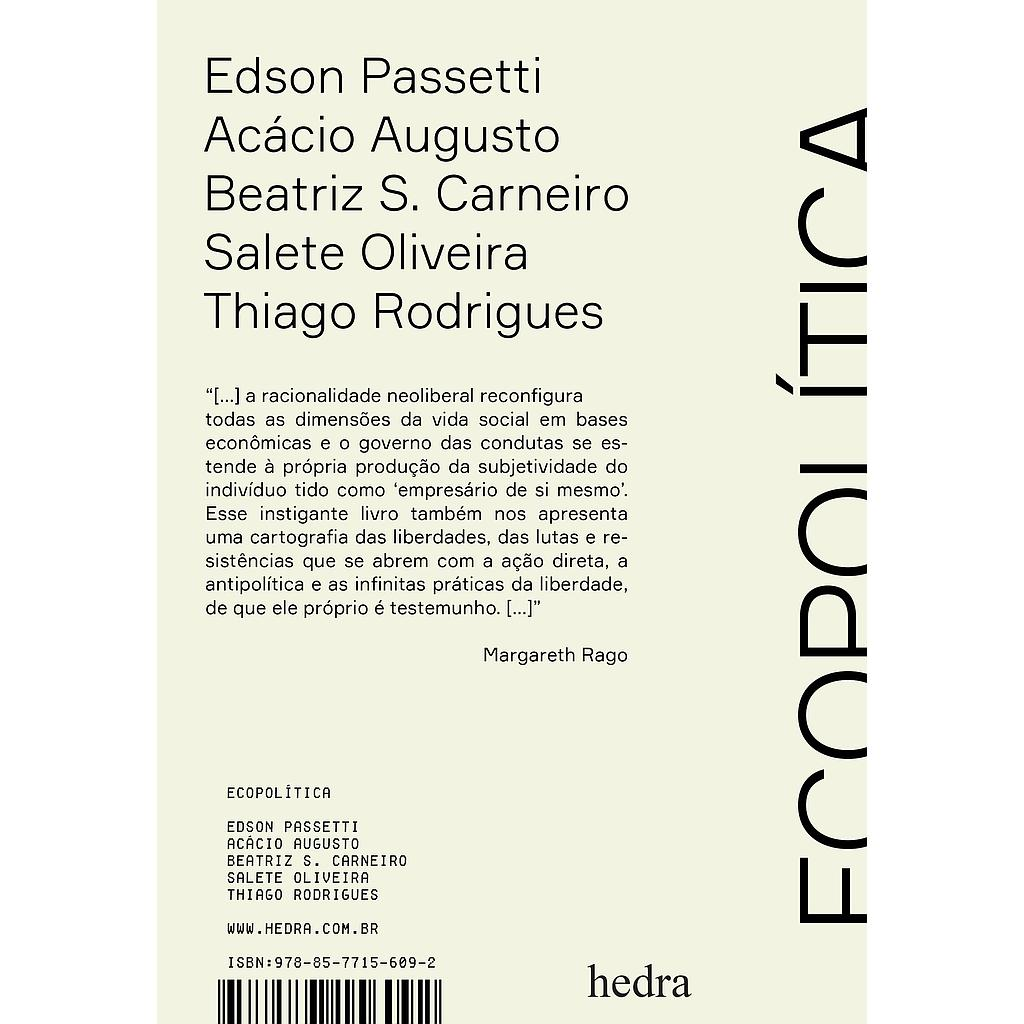
\includegraphics[width=70mm]{eco.jpeg}
\end{center}

\hspace*{-2cm}\_\_\_\_\_\_\_\_\_\_\_\_\_\_\_\_\_\_\_\_\_\_\_\_\_\_\_\_\_\_\_\_\_\_\_\_\_\_\_\_\_\_\_\_\_\_\_\_\_\_\_\_\_\_\_\_\_\_\_\_\_\_\_\_\_\_\_\_\_\_\_\_\_\_

\medskip

\noindent{}Grandes lideranças e pensadores indígenas estão reunidos em {\slsc{Tembetá}}. São seis entrevistas, feitas com Ailton Krenak, Álvaro Tukano, Biraci Yawanawá, Eliane Potiguara, Jaider Esbell e Sônia Guajajara. É o primeiro volume de uma série que busca traçar um panorama plural do pensamento indígena contemporâneo, potencializando a voz dos povos originários em detrimento de uma fictícia e embolorada história dos “conquistadores”.

\hspace{.5cm}

\hspace*{-.4cm}\begin{minipage}[c]{0.90\linewidth}
\small{
{\Formular{\textbf{
\hspace*{-.1cm}Título: Tembetá\\
Autor: Sergio Cohn e Idjahure Kadiwéu (org.)\\ 
Editora: Azougue\\
Páginas: 206\\
Formato: 14x21cm\\
Preço: R\$ 45,90\\
ISBN: 978-85-7920-228-5
}}}}
\end{minipage}


\pagebreak

\hspace{.5cm}

\begin{center}
\hspace*{-1cm}\raisebox{5.5cm}{\rotatebox[origin=t]{90}{\Formular{\textbf{Lançamento}}}}
\hspace*{1cm}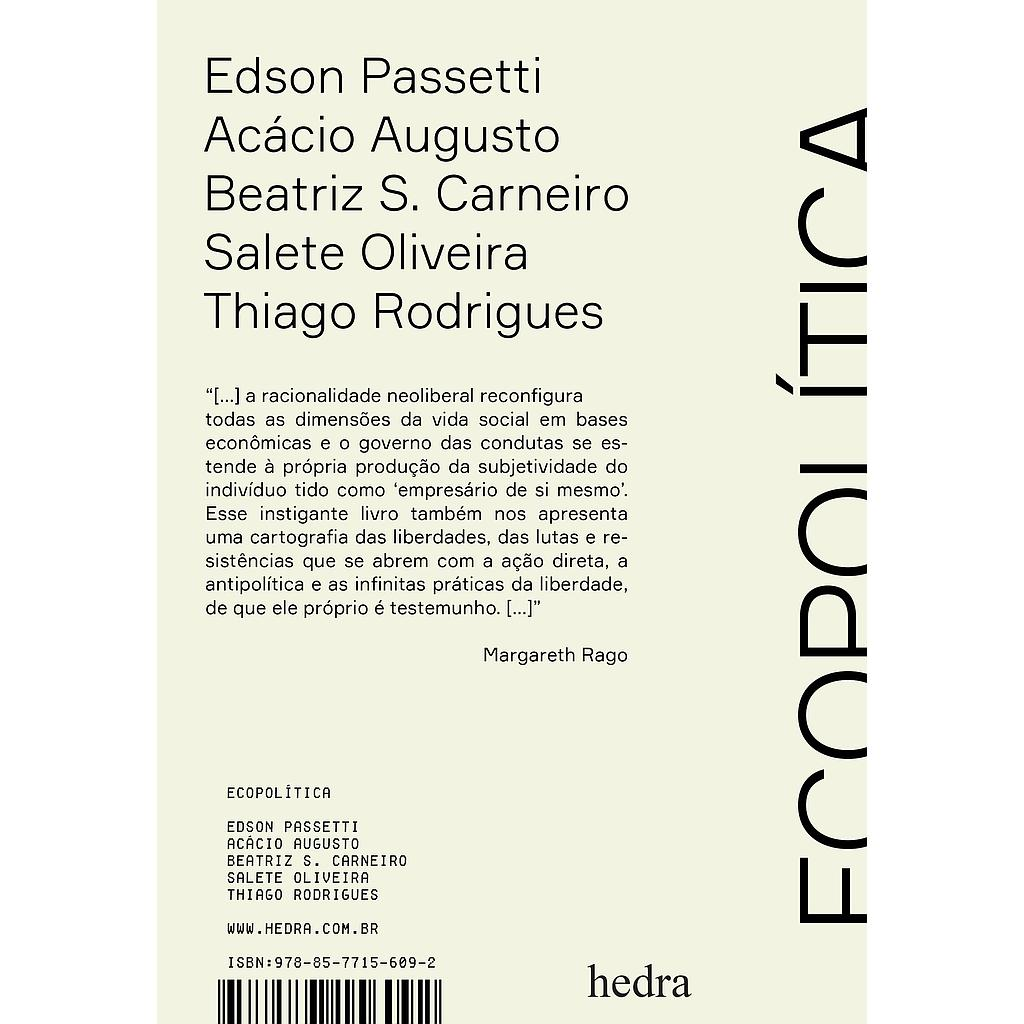
\includegraphics[width=70mm]{eco.jpeg}
\end{center}

\hspace*{-2cm}\_\_\_\_\_\_\_\_\_\_\_\_\_\_\_\_\_\_\_\_\_\_\_\_\_\_\_\_\_\_\_\_\_\_\_\_\_\_\_\_\_\_\_\_\_\_\_\_\_\_\_\_\_\_\_\_\_\_\_\_\_\_\_\_\_\_\_\_\_\_\_\_\_\_

\medskip

\noindent{}Publicado originalmente em 1962, {\slsc{Deus da Chuva e da Morte}}, livro de estreia de Jorge Mautner, alcançou grande repercussão tanto de crítica como de público, conquistando o Prêmio Jabuti daquele ano e o consagrando como um dos autores mais singulares da literatura brasileira da época.

\hspace{.5cm}

\hspace*{-.4cm}\begin{minipage}[c]{0.90\linewidth}
\small{
{\Formular{\textbf{
\hspace*{-.1cm}Título: Mitologia do Kaos (Volume 1)\\
Autor: Jorge Mautner\\ 
Editora: Azougue\\
Páginas: 488\\
Formato: 16x23cm\\
Preço: R\$ 59,90\\
ISBN: 978-85-7920-234-6
}}}}
\end{minipage}

\pagebreak
